\section{Update}\label{model-update}
Before discussing sampling, this section discusses how to update a model.
The sampling framework will naturally follow from this update procedures.
This section assumes that the detector in the previous section has selected 
a set of candidate records $R_{dirty}$ and the sampler has sampled from this
set of candidate records.
This section show that this model update procedure can be interpreted as a Stochastic 
Gradient Descent (SGD) algorithm, which gives a theoretical framework to analyze
convergence and bound the error at each step.

\subsection{Update Problem}
Let $S_{dirty} \subseteq R_{dirty}$  be a random sample of data from the results of the detection in the previous section, and let $p(r)$ be the sampling probability of each record.
The cleaner applies the data cleaning technique to the sample resulting in $S_{clean}$ and clean features and labels $(X^{(c)},Y^{(c)})$. 
In the model update problem, the updater has to update the dirty model $\theta^{(d)}$ based on the clean sample and return $\theta^{new}$.
The goal is that these updates should minimize the error of the updated model and the true model $\theta^{(c)}$ (if entire data is cleaned):
\[
error(\theta^{new}) = \| \theta^{new} - \theta^{(c)} \|
\]

\subsection{Geometric Interpretation}
The update algorithm intuitively follows from the convex geometry of the problem.
Consider this problem in one dimension (i.e., the parameter $\theta$ is a scalar value), so then the goal is to find the minimum point ($\theta$) of a curve $l(\theta)$.
The consequence of dirty data is that the the wrong loss function is optimized.
Figure \ref{update-arch2}A illustrates the consequence of this optimization.
The brown dotted line shows the loss function on the dirty data.
Optimizing this loss function finds $\theta$ that at the minimum point.
However, the true loss function (w.r.t to the clean data) is in blue.
This optimal value on the dirty data is a suboptimal point on clean curve.

\begin{figure}[ht!]
\centering
 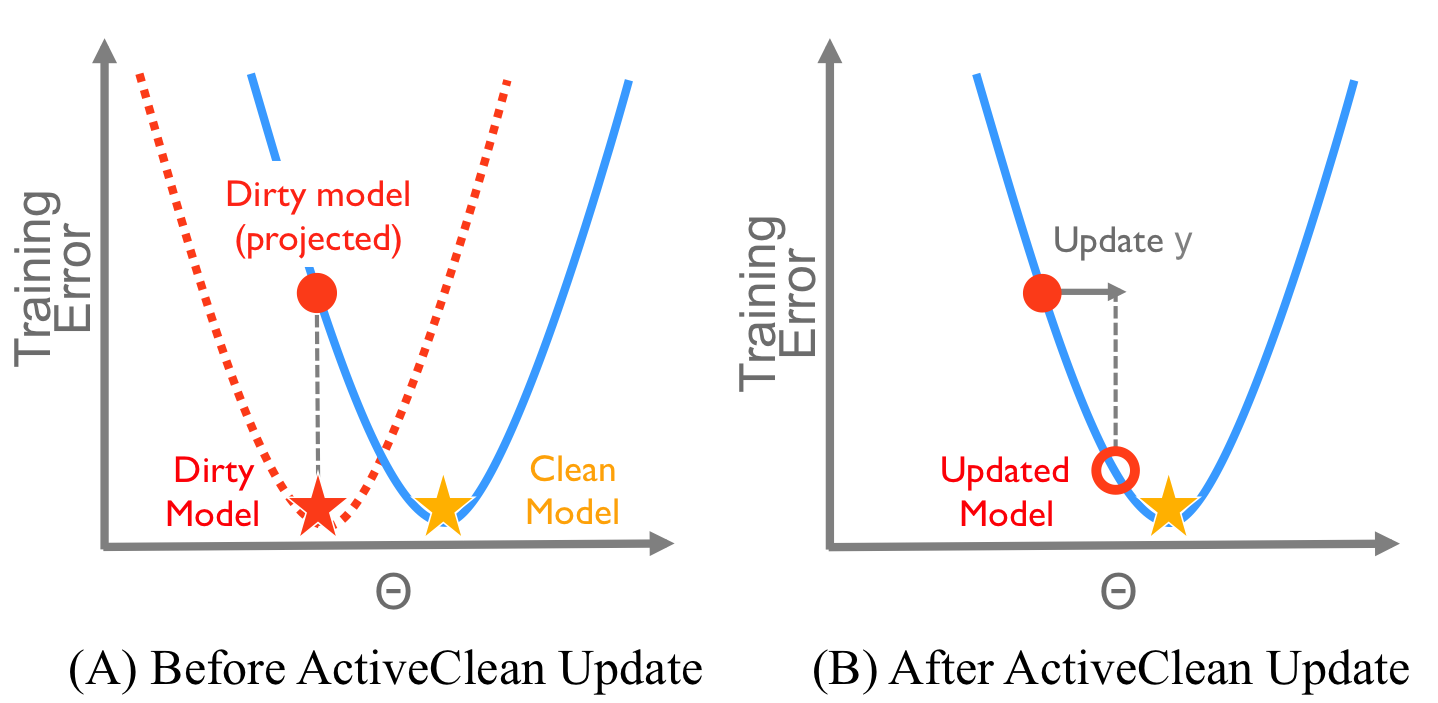
\includegraphics[width=0.7\columnwidth]{figs/update-arch2.png}
 \caption{(A) A model trained on dirty data can be thought of as a sub-optimal point w.r.t to the clean data. (B) The gradient gives us the direction to move the suboptimal model to approach the true optimum. \label{update-arch2}}
\end{figure}

The optimal clean model $\theta^{(c)}$ is visualized as a yellow star.
The first question is which direction to update $\theta$ (i.e., left or right).
For this class of models, given a suboptimal point, the direction to 
the global optimum is the gradient of the loss function.
The gradient is a $d$-dimensional vector function of the current model $\theta$ and the clean data.
Given this direction, the updater needs to update $\theta^{(d)}$ some distance $\gamma$ (Figure \ref{update-arch2}b):
\[
\theta^{new} \leftarrow \theta^{(d)} - \gamma \cdot \nabla\phi(\theta^{(d)})
\]
At the optimal point, the magnitude of the gradient will be zero.
So intuitively, this approach iteratively moves the model downhill, or corrects the dirty model until the desired accuracy is reached.

However, the gradient depends on all of the clean data which is not available and the updater will have to approximate this gradient from a sample.
The intuition, formalized in Section \ref{sgd}, is that if the gradients are on average in the right direction, the algorithm is guaranteed to converge with bounds on the convergence rate.

\subsection{Average Gradient From a Sample}
To derive a sample-based update rule, the most important property is that sums commute with derivatives and gradients.
The convex loss class of models are sums of losses, so given the current best model $\theta$, the gradient $g^*(\theta)$ is:
\[
g^*(\theta) = \nabla\phi(\theta) = \frac{1}{N} \sum_i^N \nabla\phi(x_i^{(c)},y_i^{(c)},\theta)
\]
Therefore, the gradient can be estimated from a sample by taking the gradient w.r.t each record, and re-weighting the average by their respective sampling probabilities.
Let $S$ be a sample of data, where each $i \in S$ is drawn with probability $p(i)$:
\[
g^*(\theta) \approx g_{S}(\theta) = \frac{1}{n\mid S \mid} \sum_{i \in S}\frac{1}{p(i)}\nabla\phi(x_i^{(c)},y_i^{(c)},\theta)
\]
Now adding iteration, for every batch of data cleaned $t$, the update to the current best model estimate is:
\[
\theta^{(t+1)} \leftarrow \theta^{(t)} - \gamma \cdot g_{S}(\theta^{(t)})
\]

The detection in the previous step adds a small complication, since the sample $S_{dirty}$ is not representative of all of the data.
This requires a compensation for this bias by averaging this estimate with the gradient of the complement:
\[
g_C(\theta) = \frac{1}{\mid R - R_{dirty}\mid}\sum_{i \in R - R_{dirty}}\nabla\phi(x_i^{(c)},y_i^{(c)},\theta)
\]
Then, for weights $\alpha,\beta$ (discussed in Section \ref{sgd}):
\[
g(\theta) = \alpha \cdot g_C(\theta) + \beta \cdot g_S(\theta)
\]
Finally, adding in the iteration, and at each iteration $t$, the update becomes:
\[
\theta^{(t+1)} \leftarrow \theta^{(t)} - \gamma \cdot g(\theta^{(t)}) \blacksquare
\]

\subsection{Model Update Algorithm}
To summarize, the algorithm is initialized with $\theta^{(1)} = \theta^{(d)}$ which is the dirty model.
At each iteration $t=\{1,...,T\}$, the cleaning is applied to a batch of data $b$ selected from the set of candidate dirty records $R_{dirty}$.
Then, an average gradient is estimated from the cleaned batch and the model is updated.
Iteration continue until $k = T \cdot b$ records are cleaned.

\begin{enumerate}[noitemsep]
	\item Calculate the gradient over the sample of clean data and call the result $g_S(\theta^{(t)})$
	\item Calculate the average gradient over all the data in $R_{clean}=R-R_{dirty}$, and call the result $g_C(\theta^{(t)})$
	\item Apply the following update rule:
	\[
	\theta^{(t+1)} \leftarrow \theta^{(t)} - \lambda \cdot(\alpha\cdot g_S(\theta^{(t)}) + \beta \cdot  g_C(\theta^{(t)}))
	\]
\end{enumerate} 

\noindent To summarize the parameters $b$, $\lambda$, $\alpha$, $\beta$.

\vspace{0.25em}

\noindent\textbf{Batch Size $b$ : } The batch size $b$ controls the frequency of iteration. Larger batches provide a more accurate estimate of the gradient at each iteration but has less frequent model updates. 

\vspace{0.25em}

\noindent\textbf{Step Size $\gamma$ : } $\gamma$ controls how far should to travel in the gradient direction.

\vspace{0.25em}

\noindent\textbf{Weights $\alpha,\beta$ : } $\alpha,\beta$ are the proportions to combine $g_S(\theta)$ and $g_C(\theta)$. 

\subsection{Analysis with Stochastic Gradient Descent}\label{sgd}
This update policy can be formalized as a class of very well studied algorithms called Stochastic Gradient Descent.
This provides a theoretical framework to understand and analyze the update rule, bound the error, and choose points to clean.
Mini-batch stochastic gradient descent (SGD) is an algorithm for finding the optimal value
given the convex loss and data.
In mini-batch SGD, random subsets of data are selected at each iteration and the average gradient is computed for every batch.
The key difference is that in traditional SGD there is no notion of dirty and clean data.

\vspace{0.25em}

\noindent\textbf{ \sys as Lazy SGD: } This update method is a variant of SGD that lazily materializes the clean value.
As data is sampled at each iteration, data is cleaned when needed by the optimization.
It is well known that even for arbitrary initialization SGD makes significant progress in less than one epoch (a pass through the entire dataset) \cite{bottou2012stochastic}.
Furthermore in this setting, the dirty model can be much more accurate than an arbitrary initialization; leading to highly accurate models without cleaning the entire data.

\vspace{0.25em}

\noindent\textbf{Deriving $\alpha$ and $\beta$: } The first problem is to choose $\alpha$ and $\beta$ such that the estimate of the gradient is unbiased. 
SGD will converge when the estimate is unbiased and the step-size is chosen appropriately.
The batch $S_{dirty}$ is drawn only from $R_{dirty}$.
Since the sizes of $R_{dirty}$ and its complement are known, it follows that the gradient over the already clean data $g_C$ and the recently cleaned data $g_S$ can be combined as follows:
\[
g(\theta^{t}) = \frac{\mid R_{dirty} \mid \cdot g_S + \mid R_{clean} \mid \cdot g_C  }{\mid R \mid}
\]
Therefore,
\[
\alpha = \frac{\mid R_{clean} \mid}{\mid R \mid}, \beta = \frac{\mid R_{dirty} \mid}{\mid R \mid d}
\]

\begin{lemma}\label{unbiased1}
The gradient estimate $g(\theta)$ is unbiased if $g_S$ is an unbiased estimate of:
\[
\frac{1}{\mid R_{dirty} \mid} \sum g_i(\theta)
\]
\end{lemma}
\begin{proof}[Sketch]
This result follows directly from the linearity of expectation (See Appendix \ref{unbiased1-deriv}).
\end{proof}

\vspace{0.25em}

\noindent\textbf{ Setting $\gamma$: } There is extensive literature in machine learning for choosing the step size $\gamma$ appropriately. $\gamma$ can be set either to be a constant or decayed over time. Many machine learning frameworks (e.g., MLLib, Sci-kit Learn, Vowpal Wabbit) automatically set learning rates or provide different learning scheduling frameworks. 
In the experiments, we use a technique called inverse scaling where there is a parameter $\gamma_0=0.1$, and at each iteration it decays to $\gamma_t = \frac{\gamma_0}{\mid S \mid t}$. 

\vspace{0.25em}

\noindent\textbf{ Convergence: } Convergence properties of batch SGD formulations have been well studied \cite{dekel2012optimal}. From the preceding analysis, the gradient estimate is unbiased and the step size is appropriately chosen. Following from these two points, convergence is ensured: 

\begin{proposition}
For an appropriately chosen learning rate $\gamma_t$, batch stochastic gradient descent will converge if $\mathbb{E}(g_S)=g^*$.
\label{unbiased}
\end{proposition}

\vspace{0.25em}

\noindent\textbf{ Convergence Rate: } The convergence rates of SGD are also well analyzed \cite{dekel2012optimal,bertsekas2011incremental,zhao2014stochastic}. 
This gives a bound on the error of intermediate models and the expected number of steps before achieving a model within a certain error. 

\begin{proposition}
For a general convex loss, a batch size $b$, and $T$ iterations, the convergence rate is bounded by $O(\frac{\sigma^2}{\sqrt{bT}})$. 
$\sigma^2$ is the variance in the estimate of the gradient at each iteration:
\[
\mathbb{E}(\|g_S - g^*\|^2)
\]
\end{proposition}

\vspace{0.25em}

\noindent\textbf{ Setting the batch size: } The batch size should be set by the user to have the desired properties.
Larger batches will take longer to clean and will make more progress towards the clean model, but will have less frequent model updates.
On the other hand, smaller batches are cleaned faster and have more frequent model updates but make less progress.
The overheads introduced by \sys are more evident at smaller batch sizes.
There are diminishing returns to increasing the batch size $O(\frac{1}{\sqrt{b}})$.
Empirically, in the experiments, batch sizes of 50 converge the fastest.
If a data cleaning technique requires a larger batch size than this, i.e., data cleaning is fast enough that the iteration overhead is significant compared to cleaning 50 records, \sys can apply the updates in smaller batches.
For example, the batch size set by the user might be $b=1000$, but the model updates after every $50$ records are cleaned.
This dissociates the batching requirements of SGD and the batching requirements of the data cleaning technique.

\vspace{0.5em}

\noindent\textbf{ Non-convex losses: } (See Appendix \ref{non-convex} for a note on such losses.)


